\chapter{Monte Carlo simulation method} \label{chp:MC}

In experimental particle physics, it is of great interest to use Monte Carlo
simulation method in designing detectors, understanding the detector responses
and comparing experimental data to theory predictions. In the work of this
thesis, we employ Monte Carlo simulation method for several reasons. First, we
need the simulated Monte Carlo event samples to determine if our current
designing detector parameters are good enough to characterize our targeted
measurement. As to the dihadron correlation measurement, it is the detector
coverage and resolution that we should take into consideration. Second, we will
rely on the Monte Carlo simulation method to evaluate the detector response
effect. Generally, this type of study is usually based on
GEANT~\cite{Brun:1978fy}. In our case, we use a simplified fast smearing method~\cite{EICsmear}.
In addition, we want to make some phenomenological predictions which are very
hard to be calculated with perturbative theory and can only be studied based on
some Monte Carlo models. In the end, with the event by event level description
of Monte Carlo generators we can estimate the statistical error, based on which
one can decide how much time it takes to make a conclusive measurement.

This chapter describes the Monte Carlo event generators we employed to simulate
physical events and also our fast smearing method used to estimate the detector response.


\section{The Monte Carlo event generator for \ep\ } \label{sec:MC_ep}
For the \ep\ collisions, we use the PYTHIA event generator~\cite{Sjostrand:2006za}. The event generation
process of PYTHIA can be summarized as follows (see Fig.~\ref{fig:PYTHIA_generation_scheme} for an example).
\begin{figure}
\centering
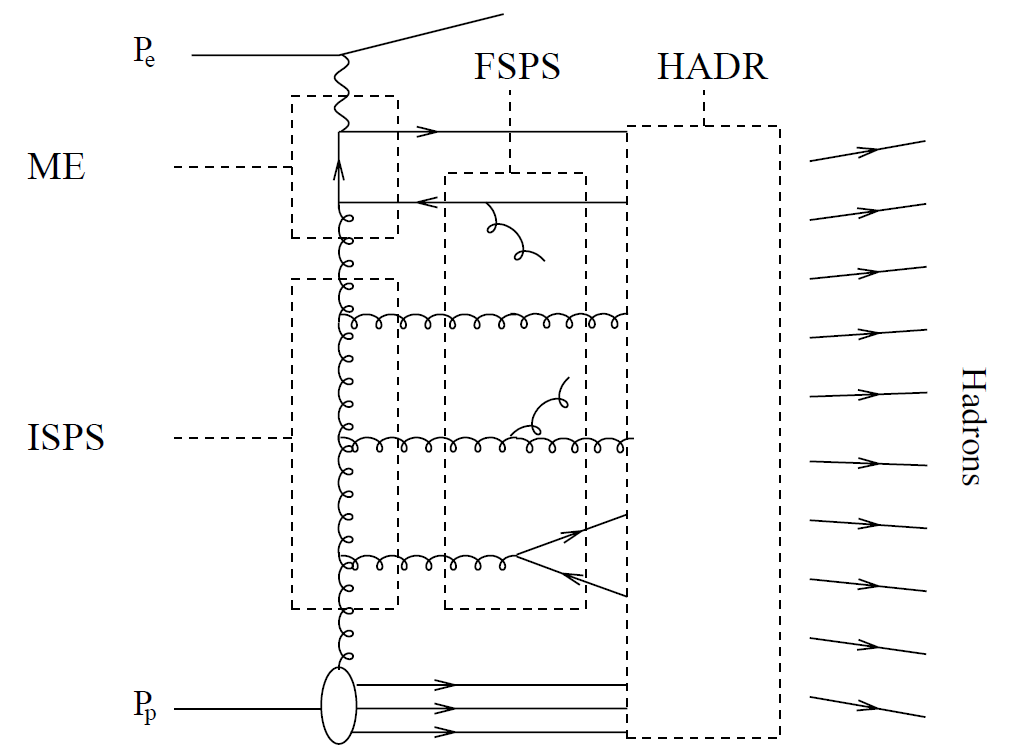
\includegraphics[width=0.7\textwidth]{plots/chpt5/PYTHIA_generation_scheme.png}
\caption[An illustration of the event generation process in PYTHIA] {
A schematic view of the event generation process in PYTHIA: hard scatering matrix element (ME), 
initial-state parton shower (ISPS), final-state parton shower (FSPS) and hadronization process (HADR). 
This plot is from Ref.~\cite{Hansson:2007zz} }
\label{fig:PYTHIA_generation_scheme}
\end{figure}
\begin{itemize}
\item Initial parton generations. The initial partons are generated depending
on the PDF description for the beam particles. The PDF sets are extracted from
a wide range of experimental tables with global fits method. It is further customary to assign a primordial transverse momentum to the initial partons, while the recoil is assumed to be taken by the beam particle remnants. 
\item Hard scattering process. The two initial partons from the beam particles may
have a hard interaction based on the matrix element for the specific Feynman diagram
determining the main kinematic feature of this event. For the PYTHIA generator, this
matrix element is calculated at the leading order.
\item Initial-state and final-state parton shower. In the parton shower model, partons
before and after hard scattering may have initial-state and final-state radiations respectively. It
is an approximation to the higher-oder QCD process at the leading-log level. 
\item Hadronization and decay process. The generated final-state partons and
beam remnants will fragment into colorless hadrons, which is a non-perturbative process
and determined from the string model~\cite{Andersson:1983ia} in PYTHIA implementation. Unstable particles decay
until reaching a set of stable final-state hadrons.
\end{itemize}

The simulation part of this study is based on the PYTHIA-$6.4$ Monte Carlo program,
with the PDF input from the LHAPDF library~\cite{Whalley:2005nh} and JETSET string model used for
hadronization processes. 


The PYTHIA Monte Carlo generator is a general purpose Monte Carlo program developed to simulate a wide range of physics process. It can be well tuned to describe the data from various experiments. This is why we use PYTHIA for the simulation of \ep\ events.


\section{The Monte Carlo generator for \eA\ }

As is known to all, we have a rich set of \ep\ Monte Carlo event generators, but
unfortunately a less favorable case for \eA~\cite{Boer:2011fh}.
DPMJET~\cite{Roesler:2000he} is believed to be one powerful generator to fit
into the simulation task for \eA\ collisions. DPMJET is treating the eA
interaction based on individual photon nucleon events simulated by
PHOJET~\cite{Engel:1994vs} in Gribov-Glauber multiple scattering
formalism~\cite{Engel:1996yb}. In the individual photon nucleon interactions a
photon is assumed to be divided into a direct photon part and a hadronic part. The
description of hadronic photon on nucleon is based on the Generalized Vector
Dominance Model (GVDM). Direct photon events include Photon Gluon Fusion (PGF)
and QCD Compton (QCDC) process. A steady transition is allowed between direct
and hadronic photon events~\cite{Roesler:1998wy}. Meanwhile, we notice that
since PHOJET, the code responsible for the elementary interaction generation in
DPMJET, only describes the interaction involving photons at very low $Q^2$ ($Q^{2}\rightarrow 0$), which indicates 
this DPMJET code allows mainly the simulation of
photoproduction off nuclei. Clearly, for the study of saturation physics, we can not use a event generator
mainly developed to simulate photoproduction events. 

Considering the fact that PHOJET responsible for treating elementary photon
nucleon interaction is quite a standalone part in the whole DPMJET framework, it
occurs to us that if we can switch the part treating photon nucleon interaction
from PHOJET to some more multi-purposed package like
PYTHIA~\cite{Sjostrand:2006za}, we can largely enforce the ability and broaden
the applicable scope of DPMJET, for example to simulate the kinematics region
covered by a proposed EIC.

Within the flexible program design of PYTHIA, we are also allowed to implement
more features such as the nuclear PDF and energy loss effect in cold nuclear
matter to accommodate the non-saturation nuclear effect. 
With everything assembling together, we can build a hybrid Monte Carlo generator reusing existing
code of DPMJET and PYTHIA at different levels with EPS09 nuclear PDF~\cite{Eskola:2009uj}
and the cold nuclear medium energy loss effect~\cite{Salgado:2003gb}. The physical process of an \eA\ collision is
generated as follows:

\begin{itemize}
    \item To begin with, a nucleon is sampled from the whole nucleus according to the nuclear geometry implemented in DPMJET.
    \item The elementary interaction of the incoming electron and the selected nucleon will be simulated according to the modules as described in PYTHIA (see Sec.~\ref{sec:MC_ep}).
    \item Before JETSET (the package responsible for parton fragmentation in PYTHIA) takes care of the final parton system in the last step, a cold nuclear medium energy loss effect will be performed to the hard scattering partons. 
    \item As we already have the particles generated for the elementary interaction from PYTHIA, we will dump the whole particle system to DPMJET, where an intranuclear cascade will happen.
    \item To close it up, the FLUKA generator~\cite{Ferrari:1995cq} which already connected with DPMJET will be used to produce deexcitation photons, nuclear fragments and some heavy remnants from the broken nucleus.
\end{itemize}

\begin{figure}
\centering
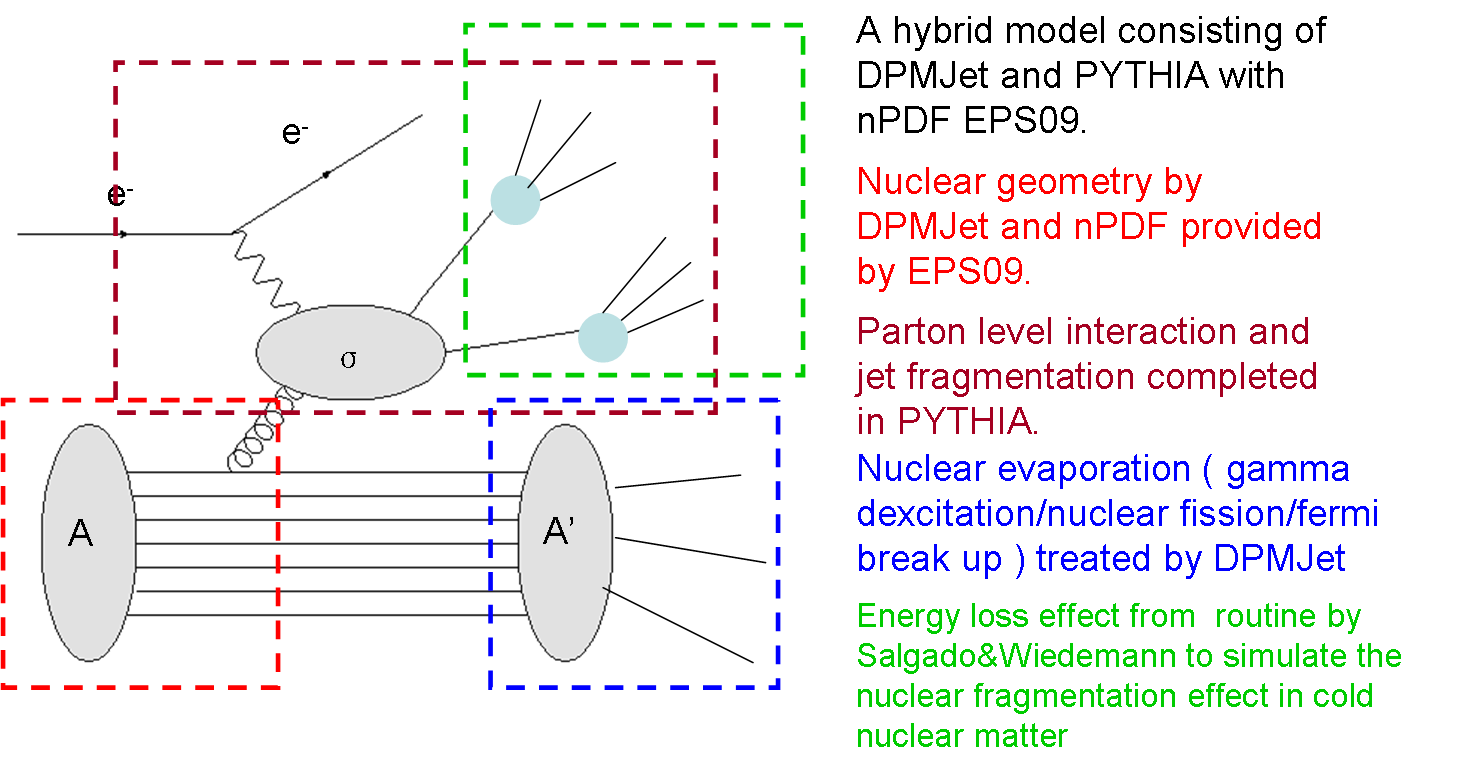
\includegraphics[width=1.0\textwidth]{plots/chpt5/eA_hybrid_chart.png} 
\caption[An illustration of the hybrid \eA\ Monte Carlo generator design layout] {
An illustration of the hybrid \eA\ Monte Carlo generator design layout. }
\label{fig:MC_hybrid_chart}
\end{figure}

The physical generation flow can be visualized in Fig.~\ref{fig:MC_hybrid_chart}.
In this model we have two significant non-saturation based nuclear effects implemented which are relevant to the dihadron correlation studies: the nuclear PDF and the cold nuclear medium energy loss effect.

\subsection{Nuclear parton distribution function}
In the hybrid Monte Carlo generator, we use a next-to-leading order (NLO) global
DGLAP analysis of nuclear parton distribution function (PDF) and their uncertainties with the release called
EPS09. Process independent PDFs of free and bound nucleons
have been discovered to be mutually different for well over twenty years. There
exist various groups offering parameterizations of the nuclear modified PDFs~\cite{Hirai:2004wq,deFlorian:2003qf}.
The nuclear modifications relative to the free nucleon PDFs are commonly named
according to the different x-regions as follows: (a) shadowing; a suppression at
$x\lesssim 0.1$, (b) antishadowing; excess around $0.1\lesssim x \lesssim 0.3$,
(c) EMC effect; depletion between $x\simeq 0.3$ and $x \simeq 0.7$, (d) Fermi
motion; an excess towards $x=1$. While the quark antiquark densities are
relatively well constrained, the modifications to gluon distributions are not
directly measured. Current nPDF parametrizations give wide variations in the
nuclear gluon densities especially in the small $x$ region due to the lack of the
nuclear DIS data in the corresponding region. However, hopefully with the advent
of the EIC era, the gluon density uncertainty can be largely constrained.

In the framework of EPS09 PDF analyses, nuclear PDF is defined with the following form
\begin{equation}
f^{A}_{i}(x, Q^{2}) \equiv R^{A}_{i}(x, Q^{2})f^{p}_{i}(x, Q^{2}),
\end{equation} 
where $R^{A}_{i}$ is the nuclear modification factor multiplied on top of the
free proton PDF $f^{p}_{i}(x, Q^{2})$ for a parton of flavor $i$, 
with $f^{p}_{i}(x, Q^{2})$ being the CTEQ6.1M PDF set. 


Assuming isospin symmetry for protons and neutrons, the up/down quark
distribution can be obtained by average according to the corresponding mass
number $A$ and charge number $Z$.


\subsection{Cold nuclear medium energy loss} \label{sec:energy_loss}
The fragmentation is another piece needs to be modified by the nuclear effect
apart from that on the parton distribution function as in nuclear deep inelastic
scattering process. Because of the non-perturbative nature of hadronization, it
is impossible to be obtained directly from the first principle calculations. People have
to rely on the phenomenological models fitted to data to describe it. The models
are based on the following aspects: hadron absorption, parton energy loss and medium
modified fragmentation function. Hadron absorption models employ formation
times and absorption cross sections for the hadrons produced in the nuclear
environment, while parton energy loss models usually use QCD inspired
calculations characterizing gluon emission off highly virtual hard partons in
the nuclear environment.

In the hybrid Monte Carlo generator, a hard parton energy loss effect is
included following the Parton Quenching Model
implementation~\cite{Dupre:2011afa} based on the extended BDMPS
calculations~\cite{Salgado:2003gb}. The parton energy loss model is originally
focused on heavy ion collisions and the characterization of quark-gluon plasma
(QGP). But it can be easily transportable to nuclear DIS case from which better
determined initial conditions can be extracted providing Based on the knowledge
of the extracted initial conditions, a precise comparison with experiments
involving heavy ion collisions can be made to describe the formation of the QGP.

In the energy loss picture, a medium is described by its transport coefficient $\hat{q}$,
defined as the average medium induced transverse momentum square per unit path
length of a hard parton:
\begin{equation}
\hat{q} = \left\langle k^{2}_{\perp}\right\rangle _{medium}/\lambda,
\end{equation}
where $\lambda$ is the mean free path and $k_{\perp}$ denotes the transverse
momentum of the emitted gluon. The characteristic energy loss scale is set by:
\begin{equation}
\omega_{c} = \frac{1}{2}\hat{q}L^{2}.
\end{equation}
As the constraint on transverse momentum $k_{\perp}$ must be smaller than the
total energy, a dimensionless quantity $R$ is introduced:
\begin{equation}
R = \frac{2\omega^{2}_{c}}{\hat{q}L} = \omega_{c}L.
\end{equation}
$L$ is the path length that parton traverses in the medium, determined by the
coordinate of the nucleon involved in certain hard interaction sampled from
a Woods-Saxon nucleus geometry. To consider the nuclear medium geometry, all we
have to do is to average over the density profile of the matter traversed by the
parton. The probability for a parton to lose energy $\Delta E$ through $n$ gluon emissions can be
written as:
\begin{equation}
P(\Delta E)=\sum^{\infty}_{n=0}\frac{1}{n!}[\prod^{n}_{i=1}\int d\omega_{i}\frac{dI(\omega_{i})}{d\omega}]
\times(\Delta E-\sum^{n}_{i=1}\omega_{i})\exp[-\int d\omega\frac{dI}{d\omega}],
\end{equation}
where $\omega_{i}$ is the emitted gluon energy and the gluon energy spectrum $\frac{dI}{d\omega}$
depends on the parameters we defined above. The probability has a discrete part and
a continuous part as follows:
\begin{equation}
P(\Delta E) = p_{0}\delta(\Delta E) + p(\Delta E),
\end{equation}
where $p_{0}$ is the discrete probability that no medium induced radiation
happens to the parton.

In our simulation, the generation of energy loss iterates as:
\begin{itemize}
	\item generate an event list at parton level from the Monte Carlo package;
	\item determine two input parameters, $\omega_{c}$ and $R$ by the generated event information;
	\item sample an energy loss $\Delta E$ according to the $P(\Delta E)$ determined in the last step;
	\item dump the modified parton system to the JETSET fragmentation module, which gives us the final particle list.
\end{itemize}

%The transport coefficient is set to $\hat{q}=0.5$. And for the sake of
%simplicity, we only assign an energy loss to the longitudinal direction of a
%parton.
%

\section{EIC fast smearing package}


\begin{figure}
\centering
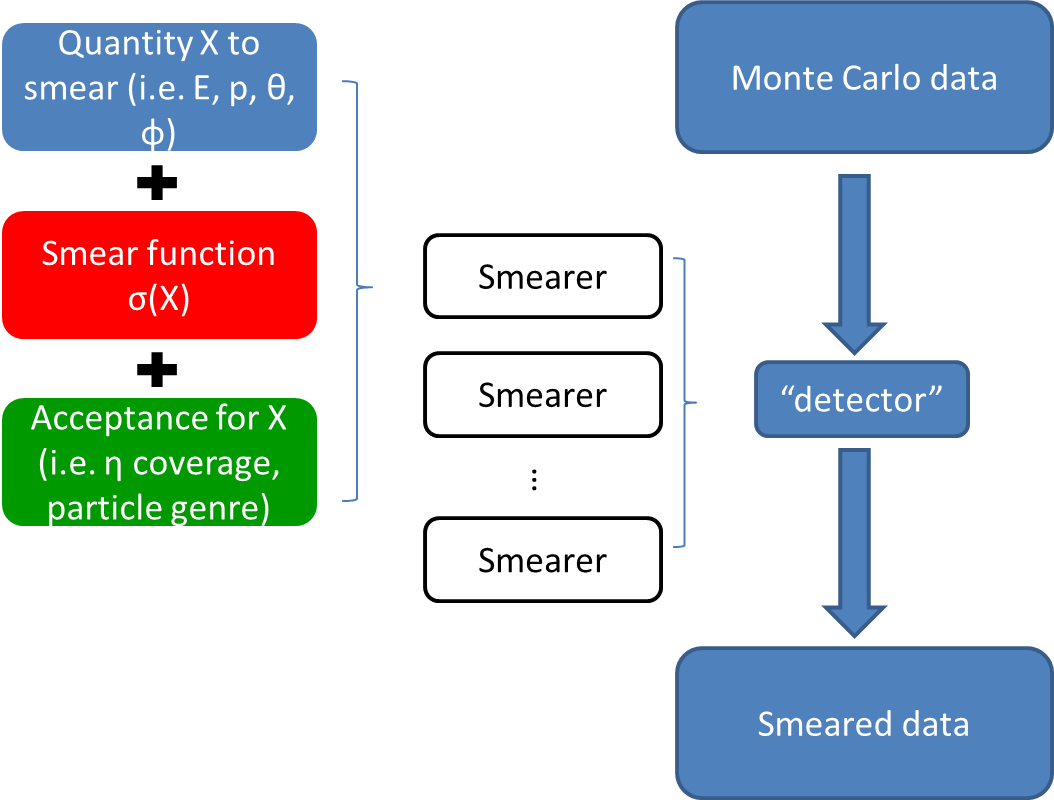
\includegraphics[width=0.8\textwidth]{plots/chpt5/smearing framework.png}
\caption[An illustration of the event smearing strategy in eic-smear package] {
A schematic view of the event smearing process implemented in eic-smear package. 
}
\label{fig:smear_layout}
\end{figure}


When a detector system tracks a particle, the information of this particle
(momentum, energy, particle id, and so on) has to be reconstructed from the electronic
signals received and analyzed at the detector read out. How well the particle
information can be reconstructed or manifested at the detector read out is
estimated by the detector resolution. The detector with a better resolution
can reconstruct particle information closer to the true value. On
the other hand, to build a detector with very high resolution will cost a lot
of budget. To make the most cost-effective design, we need to know what kind
of detector resolution is good enough to manifest the targeting physical message.

The fast smearing method implemented in the eic-smear package is a systematic
way to study the effects of detector resolution economically. The eic-smear
package provides a means for applying detector smearing to the Monte Carlo
data, whereby kinematic properties from the Monte Carlo simulated particles are modified according
to a description of the detector performance. The package contains a series of
classes and functions to facilitate the smearing of ROOT trees created from
Monte Carlo event generator. It is intended to be extremely flexible,
allowing you to change what type of smearing you want to simulate quickly and
painlessly.

As implemented in eic-smear, it is much faster to run than a full detector
simulation (e.g. GEANT), both in terms of user time spent specifying the
detector properties and in CPU time spent processing events. However,  the
smearing code is not intended as a replacement for full detector simulations.
Rather, it is a complimentary tool for roughly assessing the impact of changes
in detector performance on a physics measurement, in a way that is much more
rapid, but less detailed, than a full detector simulation. It is designed to
answer questions like given a known detector resolution, how well can we
measure some physics variables. 

\begin{table} 
\centering 
\begin{tabular}{| l | c | c | } \hline
Device	& Acceptance & resolution \\ \hline
Barrel tracking  	&  $|\eta|<1.5$  &  $\sigma_{p}/p=0.1\%$   \\  
Endcap tracking    &  $1.5<|\eta|<3$  &   $\sigma_{p}/p=1\%$   \\  
ECal   & $-1<\eta<4.5$  &  $\sigma_{E}/E=12\%/\sqrt{E}$   \\  
ECal  & $-4.5<\eta<-1$ & $\sigma_{E}/E=1.8\%/\sqrt{E}$   \\ 
HCal  & $2<\eta<4.5$ & $\sigma_{E}/E=38\%/\sqrt{E}$   \\ \hline
\end{tabular} 
\caption[The
assumed resolution for the devices to be used in our dihadron correlation simulations]{The
assumed resolution for the devices to be used in our dihadron correlation simulations.}
\label{tab:EIC_smear} 
\end{table}


In this method, a virtual device ``smearer" is defined to smear a physical
quantity $X$ according to the user specified resolution if the particle is accepted
within the smearer's coverage as shown in Fig.~\ref{fig:smear_layout}. A smearer should not necessarily be considered to
be a direct analogue of a single real-world detector subsystem (though in some
cases it may be). Rather, it is a more abstract representation of some element
of the whole detector's performance. For example, while a user may define a
single device object for smearing momentum, this device may represent the
combined tracking performance and acceptance of a number of physical detector
subsystems.

We customized a simple smearing detector for our dihadron correlation
measurement based on the EIC model detector geometry setup. The assumed
resolutions for these devices are listed in Tab.~\ref{tab:EIC_smear}.




